%!TEX root = ../dissertation.tex
\chapter{Introduction}
\label{introduction}

In the last years the scientific community made significant progress
in the development of models for solving computer vision and natural
language processing tasks. The reasons behind those outstanding
advancements are manifold. In first place, the constant increase of
computational resources allows to exploit complex models which can
capture intricate behaviour. Secondly, the availability of new data
speed-up the learning process in terms of how we can benefit from
available information. However, the joint understanding of both
modalities is still an hard task, specially if we constraint the
problem within a deliberately simple and human-like environment.

Both visual and language modalities are required for solving
interesting, challenging and community worthwhile problems such us
visual question answering, image retrieval, robotic navigation and
visual grounding \todo{CITE PAPERS}. Among these, visual grounding
task is a foundamental building block and can be used to postulate
other tasks as a variation of the latter. A first abstract definition
for visual grounding could be:

\begin{quote}
    \textit{The task of locating the content of the image referenced
    by a given sentence.}
\end{quote}

With the availability of large datasets \todo{CITE DATASET PAPERS},
many different solution for the visual grounding task has been
proposed in literature, but most of them relies on expensive
annotations. We argue that this technique cannot scale and is becoming
a critical bottlenck: it is hard and expensive to collect grounding
information while very simple to collect images with their
descriptions. Also, the way humans learn phrase localization is by
assembling prior kwnowledge instead of memorize a mapping between
textual and image examples.

This encourages us to investigate the visual grounding task under the
weakly supervised setting. In weakly supervised scenario, the
available ground truth is a shallow information which links a
description with its own image and vice-versa. On the countraty, the
fully supervised setting provide also the information between noun
phrases and objects in image, while in unsupervised settings no ground
truth is available.

In this work, we propose a model for exploiting semantic information
convoyed by class labels on bounding box. We assert that, given a
phrase, the image should contain an object detected by an object
detector whose bounding box class label is similar to the head of
given phrase. \todo{rivedere la forma}

\section{Visual Grounding}

Visual grounding is the general task of locating the components of a strucutred description in an image. 

Take for example the image in Fig.~\ref{fig:dog-playing-with-ball} and
the phrase ``A collie plays with a white ball in a field of green
grass''. We can think to many solutions for the visual grounding
problem given that input. A first approach would be to grossly
localize the subject of the phrase in the image, thus, pratically
speaking, to draw a coarse box around the dog playing with the ball
(red box). Another solution instead would be to localize the ball, the
dog and the ground distinctly, identifying precise regions of the
image and draw precise boxes among interesed objects. Both two
solutions are legal and belong to the visual grounding field. The
former is known as referring expression grounding (REG) while the
latter as phrase grounding (PG). The main difference between the two
is the grain used to solve the problem, and this has significant
impacts on how we can approach the problem and the relevance for other
tasks.
\todo{add "see section XX" for more details.}

\begin{figure}
    \centering
    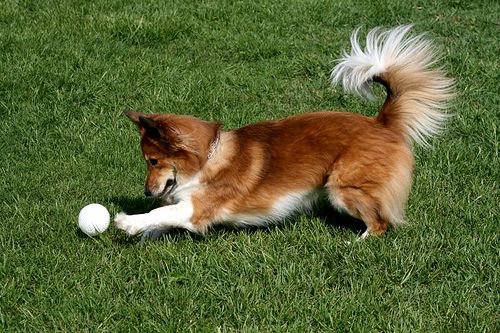
\includegraphics[width=0.7\textwidth]{resources/dog-playing-with-ball.jpg}
    \caption[Short figure name.]{This is a figure that floats inline and here is its caption. \todo{complete description and add two images, one for reg and the other for phrase grounding}
    \label{fig:dog-playing-with-ball}}
\end{figure}

\newthought{Referring Expression Grounding} is the task of locating
the subject referred by an expression in given image. 

More formally, given in input an image $\bm{I}$ and a sentence
$\mathrm{S}$, REG consists in learning a function $\delta$ from the
set $\calS$ of sentences to a set of bounding boxes $B$ defined on
$\bm{I}$, i.e., $\delta: \calI \times \calS \rightarrow 2^{\calS
\times \calB}$, where $\calI$ is the domain of images, $\calS$ is the
domain of sentences, $\calB$ is the domain of bounding boxes which can
be defined on $\calI$, and $2^{\calS \times \calB}$ is the power set
of the cartesian product between $\calS$ and $\calB$. In our example,
``the dog'' is the referred expression and the red bounding box is the
correct solution.

\newthought{Phrase Grounding}, instead, is the task that studies the
mapping from noun phrases to regions of an image. In order to solve
this task, first, it is necessary to recognize all the objects in the
image and the components in the text, while after, the model needs to
find the correct alignment among the nouns and the objects.

More formally, given in input an image $\bm{I}$ and a sentence
$\mathrm{S}$, phrase grounding consists in learning a mapping $\gamma$
from the set $\calQ$ of noun phrases to a set of bounding box $\calB$
defined on $\bm{I}$, i.e., $\gamma : \calI \times \calS \rightarrow
2^{\calQ \times \calB}$. So, given an image $\bm{I}$ containing $e$
objects identified via the set of bounding boxes $B_\calI = \{ b_i
\}^e_{i=1}$, where $b_i \in \Rset^4$ is the vector of coordinates
identifying a bounding box in $\bm{I}$, and a sentence $\mathrm{S}$
containing $m$ noun phrases gathered in the set $\calQ_S = \{ q_j
\}^m_{j=1}$, where $q_j \in \Nset^2$ is a vector containing as
coordinates the initial and final character positions in the sentence
$\mathrm{S}$, $\gamma(\bm{I}, \mathrm{S})$ returns a set of couples
$\{ (\bm{q}, \bm{b}) \mid \bm{q} \in \calQ_{\mathrm{S}}, \bm{b} \in
B_{\bm{I}} \}$ where each couple $(\bm{q}, \bm{b})$ associates the
noun phrase $\bm{q}$ to the bounding box $\bm{b}$. Please, notice that
the same noun phrase can be associated to several different bounding
boxes, as well as the same bounding box can be associated to many
different noun phrases. Following the current literature, in this
paper we assume that each noun phrase is associated to one and only
one bounding box. Bounding boxes, however, can identify more objects,
e.g. several persons in the case the noun phrase is ``people''.

Back to our example, the phrase grounding task consists in identifying
the red, blue and green bounding box enclosing, respectively, the dog,
the ball and the field of gress grass.

\newthought In of our work we will focus on phrase
grounding, as it is considered the foundamental building block for
many high-level computer vision tasks such as image retrieval, QA,
video QA, etc. \todo{cite kwnowledge aided consistency}.

\cite{conser2019revisiting} \todo{FIX CITE}

\section{Two Stage vs One Stage}

Visual grounding is a challenging task which requires the semantic
understanding of the image content and its textual description. In
order to lower the complexity of the whole task, visual grounding is
generally formulated as an object detection task followed by a
classification task in which, given an input image and sentece, the
goal is to return only the detected object(s) that represents the best
semantic match with the sentence. This approach was extensively used
by many researchers in visual grounding field \todo{CITE vedere fast
and accurate one-stage approach...} due to its simplicity. On the
other hand, some recent works started introducing the one stage
approach in which the object detection and the classification problem
are solved joinly, arguing this new architecture may lead to faster
and more accurate models.

\newthought{The two stage approach} is a simple approach to the visual
grounding task which relies on the decomposition of the main task in
two sub-tasks, namely object detection and classification. Given an
input image, the first step generates candidate regions using an
object proposal extractor such us Edge Boxes and Selective Search
\todo{CITE edge box, selective searcg} or by an object detector, such
us Faster R-CNN, Single Shot multibox Detector (SSD), or YOLO
\todo{CITE faster rcnn, ssd, yolo...}. The second step consists in
ranking this candidate regions, which hopefully capture the semantic
context, conditioned on a language query about the image. Practically,
this means that the model predicts, for each proposal bounding box, a
score that represents how much the content of the bounidng box is
likely to be referred by the sentence. Sometimes, models predict also
new coordintas for the best predicted proposal, in order to better fit
the visual content accordingly to the sentence semantic information.
\todo{Aggiungere schema che descrive l'approccio}

Even if the approach seems very promising, it is not exempt from some
problems. As reported by \todo{CITE fast and acc one stage} ``the
propose-and-rank two stage framework is flawed in at least two major
ways''. First of all, if none of the region candidates of the first
stage hits the ground truth region, the whole framework fails no
matter how good the second ranking stage could perform. Note that a
hit is considered successful if any of the proposals overlap the
ground truth by more than fifty percent in term of intersection over
union (IoU). Secondly, they argue that the process can be optimized by
focusing on relevant bounding boxes which are often a small number
(2-5), instead of waste lot of resources by computing thousands of
proposal and then rank them down to a list.

However, the highlighted problems highly depends on chosen
proposal extractor/object detector. Consider, for example, the problem
of hitting the ground truth with at least one bounding box. Given an
image $\bm{I}$ and $b'$ the ground truth bounding box, if we employee
a very simple (yet extremely inefficient) proposal extractor such us
the one who generates $\bm{B}$ the set of all possible bounding boxes
in $\bm{I}$, then, by construction we have that $b' \in \bm{B}$. So,
by chosing the maximum number of bounding box we can tackle the
problem. However, this solution is not feasible in practice, but
fortunately we do not need to generate all possible solutions. In
fact, only a small subset of all solution are required to hit the
ground truth bounding box because thanks to the advancements in object
detection system we can recognize relevant objects in image and focus
only on those proposals.

Practically, we proved that with 100 bounding boxes and Faster-R CNN
object detector, we obtain a coverage which is greater than 90\% on
both two major dataset in the field of study: Flickr30k and ReferIt.
The table \todo{REF table} shows how the upperbound accuracy changes
by varying the number of considered bounding box.

The second problem instead is partially solvable because the system,
in order to perform its classification task, needs to consider all the
extracted proposal. However, the first stage can be precalculated and
cached for the second stage, drastically reducing the required
resources. 

\newthought{The one stage approach} firstly introducted by \todo{CITE
fast and accurate one stage}, instead, relies on a single step for
computing the solution. The model receives in input an image and a
textual sentence, and it should learn how to extract and fuse all the
visual and textual information in order to predict the best bounidng
box in output, according to the input sentence. 

The thight coupling provided by this approach may lead to interesting
results \todo{CITE fast and accurate one stage}, but it raises some
major issues: \begin{enumerate*}[label=(\roman*)] \item not all the
visual grounding datasets are suitable for training an object
detector, due to lack of images and/or because they are not densely
annotated; \item the model requires an high number of parameters, and
because of that \item the training requires significant computing
resources. \end{enumerate*}

\section{Fully/Weakly/Self/Un-Supervised Settings}

Machine learning has achieved great success in various tasks,
particularly in supervised learning tasks such as classification and
regression, but it is noteworthy that in many other tasks it is
difficult to get strong supervision information like fully
ground-truth labels due to the high cost of the data-labeling process.

Visual grounding is a striking example of that. Consider again the
example with image given in Fig.~\ref{img} and the sentence "A
colly..." \todo{completare sentence copiandola da sopra}.
\todo{Valutare se cambiare esempio o meno} In order to properly
evaluate the phrase localization task, is required to know each query
$q$ \todo{aggiustare matematica} in sentence $S$, and for each query
$q$ the mapping to a bounding box $b$ in image $I$, which means to
know also bounding boxes.\todo{aggiustare forma}. Practically
speaking, a human annotator given an image $I$ and a sentence $S$ has
to annotate all queries in sentence, undestand the query, identify the
referred object in image by drowing a bounding box surrounding it and
linking the bounding box with the query. With those insight it's
straighforward to see that the fully supervised scenario for the
visual grounding task is very hard to obtain. 

More abstractly, in fully supervised settings a training example
consists of two parts: a feature vector (or instance) describing the
event/object, and a label indicating the ground-truth output.
Projected in phrase grounding this means knowing the map $\gamma :
\calI \times \calS \rightarrow 2^{\calQ \times \calB}$ that links the
ground truth bounding box $b_i \in \calB$ with its query $q_j \in
\calQ$.

Another form of supervision is the weak supervision. Broadly speaking,
weakly supervised learning is an umbrella term covering a variety of
studiesthat attemptto construct predictive models by learning with
weak supervision \todo{CITE A brief introduction to weakly supervised
learning}. Typically, there are three types of weak supervision. 

\begin{itemize}
    \item The first is incomplete supervision, i.e. only a (usually
small) subset of training data is given with labels while the other
data remain unlabeled. \todo{AKA semi-supervised, CITE grounidng by
reconstruction}. Consider the following image TODO with the sentence
TODO \todo{}, in incomplete supervision we may lack some ground truth,
i.e., not for some query $q$, $\gamma(\bm{I}, S)$ is undefined.
    \item The second type is inexact supervision, i.e. only
coarse-grained labels are given. In phrase grounding inexact
supervision means we have weak ground truth, for example given
$\bm{I}$ an image and $S$ a sentence a weak ground truth may be the
map $\gamma' : \calI \times \calS \rightarrow 2^{\calI \times \calS}$.
Note that in this setting we do not know which bounding box $b$ is
linked to query $q$. \todo{aggiustare notazione math}
    \item The third type is inaccurate supervision, i.e. the given
labels are not always ground truth.  In other words, some label
information may suffer from errors.
\end{itemize}

The third type of weakly supervision in phrase grounding is usually
mixed with the other because the label procedure which must be carried
out by an human annotator and it's very error prone.
